\documentclass[12pt]{article}

\usepackage{natbib}
\usepackage{amssymb}
\usepackage{amsmath}
\usepackage{bm}
\usepackage{dsfont}
\usepackage[margin=1.25in]{geometry}
\usepackage[font=footnotesize]{caption}
\usepackage{dsfont}
\usepackage{amsmath}
\usepackage{graphicx}
\usepackage{bm}
\usepackage{enumerate}
\usepackage[shortlabels]{enumitem}
\newcommand{\m}[1]{\mathbf{\bm{#1}}}
\newcommand{\R}{I\hspace{-4.4pt}R}
\newcommand{\bc}[1]{\textcolor{blue}{\mathbf{#1}}}
\newcommand{\ind}{\mathds{1}}

\setlength{\parindent}{0pt}

\begin{document}

AMS 268 -- Homework 1

Mickey Warner
\bigskip
\bigskip


The following table provides a summary of each of the three models: LASSO, ridge, and spike and slab. The LASSO and ridge models were fit after $10$-fold cross-validation using the \texttt{glmnet} package.
\bigskip

The spike and slab model uses a mixture of two normals for each $\beta_j$, where one component has most of its mass close to zero and the other is more dispersed. A latent variable is assigned to identify the mixture to which the $\beta_j$ belongs. A $Beta(1,1)$ prior is given for the probability class of the latent variable. An $IG(1,1)$ prior is given for the variance $\sigma^2$. This yields closed-form expressions for the full conditionals of all parameters.

\begin{table}[ht]
\centering
\begin{tabular}{r|rrr|rrrrrr}
  \hline\hline
 & \multicolumn{3}{c|}{MSPE} & \multicolumn{6}{c}{Spike and Slab} \\
 & LASSO & Ridge & Spike & $M_{nonzero}$ & $M_{zero}$
 & GOF & PEN & PPL & MSPE \\ 
  \hline
 1 & 0.98 & 0.91 & 0.79 & 0.18 & 0.17 & 393 & 551 & 945 &      \\
 2 & 0.95 & 0.93 & 0.80 & 0.21 & 0.19 & 321 & 476 & 797 &      \\ 
 3 & 0.92 & 0.56 & 0.42 & 0.21 & 0.19 & 211 & 592 & 803 &      \\ 
 4 & 0.95 & 0.46 & 0.30 & 0.24 & 0.21 & 121 & 429 & 551 &      \\ 
 5 & 1.02 & 1.04 & 0.80 & 0.25 & 0.21 & 400 & 539 & 939 & 0.63 \\ 
 6 & 1.00 & 0.99 & 0.82 & 0.28 & 0.23 & 328 & 462 & 790 &      \\ 
 7 & 0.91 & 0.64 & 0.48 & 0.30 & 0.23 & 241 & 580 & 821 &      \\ 
 8 & 0.81 & 0.54 & 0.36 & 0.32 & 0.24 & 143 & 419 & 562 &      \\ 
 9 & 0.90 & 1.14 & 0.79 & 0.18 & 0.17 & 394 & 554 & 949 &      \\ 
10 & 0.94 & 1.19 & 0.80 & 0.22 & 0.20 & 319 & 483 & 802 &      \\ 
11 & 0.88 & 0.92 & 0.42 & 0.21 & 0.19 & 212 & 591 & 803 &      \\ 
12 & 2.19 & 1.62 & 0.30 & 0.24 & 0.21 & 120 & 428 & 548 &      \\ 
13 & 3.60 & 3.37 & 0.80 & 0.27 & 0.22 & 400 & 544 & 945 &      \\ 
14 & 1.46 & 1.49 & 0.81 & 0.33 & 0.25 & 325 & 472 & 797 &      \\ 
15 & 1.62 & 1.46 & 0.48 & 0.31 & 0.23 & 241 & 584 & 825 &      \\ 
16 & 1.93 & 1.41 & 0.36 & 0.35 & 0.25 & 144 & 426 & 570 &      \\ 
   \hline\hline
\end{tabular}
\caption{Mean-squared prediction error (MSPE) for LASSO, ridge, and spike and slab, and quantities associated with the spike and slab model: $M_{nonzero}$ and $M_{zero}$ are mean h.p.d. interval lengths for true $\beta_j\neq 0$ and $\beta_j=0$, GOF is goodness-of-fit calculated as $\sum_{i=1}^n(y_i - y_{pred})^2$, PEN is a penalty $\sum_{i=1}^n \mathrm{var}(y_{pred})$, and PPL (posterior predictive loss) is the sum of GOF and PEN. The final column is MSPE of a new set of covariates.}
\end{table}


\begin{figure}
\begin{center}
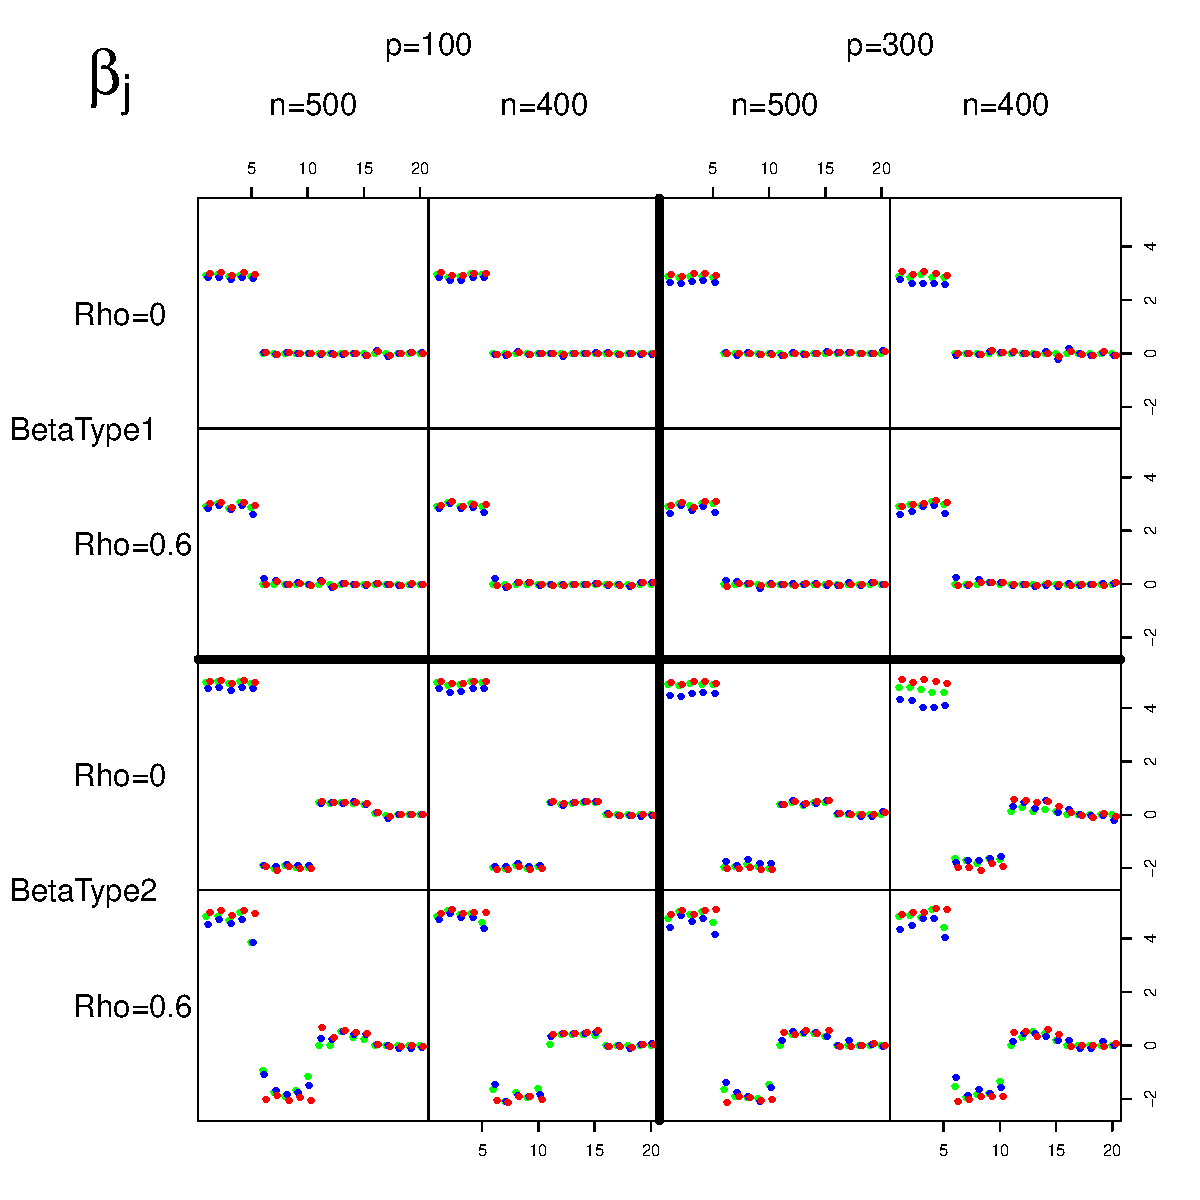
\includegraphics[scale=0.75]{figs/betas.pdf}
\end{center}
\caption{Estimates for $\beta_j$ for each of the three models for all sixteen scenarios. The first 20 $\beta_j$'s are shown (all of them afterward are close to zero). Green: LASSO. Blue: Ridge. Red: Spike.}
\end{figure}

From the MSE, we see that ridge did just as well or better than LASSO in every case, but the spike and slab did better still. In fact, for every scenario, the spike and slab model correctly identified all zero and non-zero coefficients. The LASSO would at times estimate non-zero coefficients which should be zero. Though these estimates would be small, the corresponding $p$-values would sometimes indicate a non-zero effect. Hence, the spike and slab was superior in variable selection.
\bigskip

The figure on the previous page shows the posterior mean of $\beta_j$ in the spike and slab model and the estimates from the LASSO and ridge models at each of the sixteen scenarios. We see that LASSO (green) and spike and slab (red) are in close agreement, whereas the ridge estimates tend to be slightly shrunk more towards zero. This is more apparent under BetaType2 (which 15 non-zero coefficients). The spike and slab seems to do well fairly consistently.
\bigskip

Finally, we calculated the mean-squared prediction error (MSPE) for a particular combination: $n=500$, $p=100$, $\rho=0.6$, and beta type 1. We simulated 50 new responses and covariates $(y_{pred,i}, \m{x}_{pred,i}^\top)$. We obtained the posterior predictive distribution from the spike and slab model for each of these 50 covariates and compared the mean prediction, $\hat{y}_i$, against the truth
\[ MSPE=\frac{1}{50}\sum_{i=1}^{50}(y_{pred,i} - \hat{y}_i)^2 \]
and obtained a value of $0.63$, as noted in the fifth row of Table 1. This seems pretty good considering our MSPE was higher when making in-sample predictions.

\end{document}
